\documentclass[twocolumn]{article}

% Language setting
\usepackage[english]{babel}
\usepackage{indentfirst}

% Set page size and margins
\usepackage[a4paper,top=2cm,bottom=2cm,left=2cm,right=2cm,marginparwidth=1.25cm]{geometry}

% Useful packages
\usepackage{amsmath}
\usepackage{graphicx}
\usepackage{url}
\usepackage[colorlinks=true, allcolors=blue]{hyperref}
\usepackage{natbib}

\title{Projet de deuxieme annee}
\author{Pierre P\'ebay, Ismail Benchekroun \and Encadrant : Vincent Barra, R\'ef\'erent : Jean-Philippe Gayon}

\begin{document}
\maketitle

\twocolumn

\section{Pr\'esentation}

L'utilisation de technologies informatiques dans les industries financières est un domaine r\'ecent et en pleine expansion. Elle modifie considérablement la façon dont de nombreux problèmes de prise de décision financière sont abordés, tels que ceux liés au \textit{trading} (achat et vente d'actions d'entreprise), à l'investissement, à la gestion des risques, à la gestion de portefeuille, à la détection des fraudes et au conseil financier. Le \textit{trading} algorithmique, également connu sous le nom de \textit{trading} quantitatif, est un aspect essentiel de ce d\'eveloppement et consiste à utiliser des ordinateurs et diff\'erents types d'algorithmes pour effectuer des transactions. Ces problèmes complexes de prise de décision peuvent être difficiles à résoudre en raison de leur caractère stochastique, de leur non-stationnarité, de leur non-linéarité, du bruit résultant du comportement humain irrationnel qui alimente les données et d'une observabilité du march\'e partielle. Notre objectif est d'\'etudier et d\'evelopper des algorithmes de \textit{trading}, en particulier avec des mod\`eles d'apprentissage machine.

\section{Mots-Cl\'es}


\begin{itemize}
    \item \textbf{En fran\c{c}ais:} \textit{Trading} Algorithmique, Analyse Technique, Apprentissage par renforcement profond,  Méthode policy-gradient, Bourse, Arbitrage.

    \item \textbf{En anglais:} Algorithmic \textit{Trading}, Technical Analysis, Deep Reinforcement Learning, policy gradient methods, Stock Exchange, Arbitrage.
\end{itemize}


\section{Revue de littérature}

Lorsque l'on s'introduit a la finance, quantitative ou non, le terme le plus populaire qui revient dans les recherches non académiques est celui de "\textit{technical analysis}" ou analyse technique. L'analyse technique est un grand ensemble de techniques numériques qui ont pour objectif d'analyser les séries temporelles des objets financiers étudiés, pour avoir des signaux (un dépassement de valeur, un croisement de courbes, etc.) d'action \`a prendre. Ces techniques étant très simples et n'ayant aucune barrière technique pour les appliquer, elles sont très attrayantes au débutant, d'autant plus qu'elles sont très mises en avant dans le monde non académique de la finance. Mais qu'en est-il de l'efficacité de ces méthodes ? Il s'agit d'un sujet très débattu, certains assurant leur réussite avec ces méthodes tels \cite{hsu_technical_2016}, d'autres expriment leur doute tels \cite{marshall_can_2008} qui expliquent les réussites par des biais de sélections et autres erreurs d'analyse statistique.
\newline

Une autre approche plus académique est celle de la modélisation sans connaissances préalables nécessaires sur la construction du marche financier, avec des techniques de régression et d'apprentissage machine qui. Il y a cepandant un probl\`eme majeur avec ces mod\'eles en raison de leur incapacit\'e \`a apprendre les d\'ependance \`a long terme \`a cause du fameux problème du gradient de fuite \cite{bao_deep_2017}. Pour r\'esoudre ce probleme, Hochreiter et Schmidhuber ont introduit en 1997 les cellules \`a m\'emoire interne (LSTM) \cite{gers_learning_2000} pour leurs capacit\'e \`a r\'eguler leurs propre m\'emoire en utilisant un m\'ecanisme de blocage qui apprend quelles informations à conserver, à transmettre et à oublier. Il est largement utilisé et a démontré d'excellentes capacités de prédiction dans le traitement du langage naturel,la reconnaissance de l'écriture, la reconnaissance des d'images et le sous-titrage d'images \cite{byeon_scene_2015}. En finance, les LSTM ont \'et\'e de plus en plus utilis\'e  pour l'analyse des s\'eries temporelles. Par exemple, les applications pour les pr\'edictions de prix sur les principaux indices boursiers du monde entier tels que le S&P500, l'indice SSE de Shanghai, le NIFTY 50 en Inde et l'Ibovespa au Brésil \cite{bao_deep_2017}.
\newline

\cite{theate_application_2021} propose l'algorithme Trading Deep Q-Network (TDQN), une approche d'apprentissage par renforcement profond du problème de la détermination de l'action de \textit{trading} optimale sur les marchés boursiers. L'algorithme TDQN est entraîné à l'aide de données boursières historiques pour générer des scénarios artificiels, que l'algorithme utilise pour apprendre les stratégies de \textit{trading} optimales. L'apprentissage est entièrement basé sur les données, ce qui signifie qu'il ne nécessite pas l'utilisation de règles explicites pour prendre des décisions de \textit{trading}. Cela rend l'algorithme TDQN très polyvalent et capable de s'adapter à différents marchés financiers.
\newline

Les performances de l'algorithme TDQN ont été évaluées à l'aide d'une nouvelle méthodologie d'évaluation des performances, qui a montré que l'algorithme surpasse les stratégies de \textit{trading} de référence. L'algorithme TDQN s'est également avéré robuste aux divers coûts d'intermediaires, ce qui signifie qu'il est capable de s'adapter à différents types d'environnements de \textit{trading}.
\newline

Plusieurs directions pour les recherches futures sont sugg\'er\'ees. L'une d'entre elles consiste à améliorer l'observabilité de l'environnement de \textit{trading} en incluant des donn\'ees telles que le taux d'inflation, ce qui permettrait à l'algorithme TDQN de prendre des décisions plus éclairées. Un autre domaine de recherche consiste à utiliser le m\^eme apprentissage par renforcement avec attribution de la r\'ecompense non plus en fonction de la variation de valeur de la position mais en fonction de la maximisation du ratio de Sharpe. Dans l'ensemble, l'algorithme TDQN présente des résultats prometteurs et est un mod\'ele int\'eressant pour le \textit{trading} algorithmique.
\newline

Une autre approche est celle de \cite{park_practical_2021} qui utilisent les m\'ethodes d'apprentissage renforc\'e "State-Representation" et d'apprentissage par imitation, en utilisant que des positions dites "longues" de \textit{trading}. En effet les positions dites "courtes" de \textit{short selling} n\'ecessitent des privil\`eges sp\'ecifiques, notamment des comptes sur marge, et entra\^inent des co\^uts de transactions \'elev\'es.
\newline


\section{Définition du problème financier}

L'hypothèse de l'efficience du marche des capitaux, ou \textit{efficient market theory}, énonce que tous les prix de tous les actifs de ce marche reflètent la valeur intrinsèque des sujets de ces actifs. Autrement dit, le prix reflète la valeur. Dans le march\'e des actions d'entreprises, cette théorie n'est pas applicable, les prix ont de fortes variations autour du prix reflétant la valeur, ce qu'on appelle "volatilité".
L'objectif du \textit{trader} est alors de profiter de cette inefficacité du marche, donc acheter l'action au prix inférieur du prix réel de la valeur, et vendre a un prix supérieur afin de générer du profit.
\newline

Dans le cadre de notre projet, nous ne nous intéresserons qu'au problème simple des parts d'entreprises, dites "actions", que nous pourrons, de façon hypothétique, vendre et acheter instantanément. En réalité, le temps entre la décision d'acheter ou de vendre est significatif en raison du passage par le courtier, qui doit trouver des vendeurs et des acheteurs correspondants. Le passage par ce courtier ainsi que tous les autres intermédiaires nécessaires a agir dans le marche vont impliquer des coûts de transactions, que seront a considérer dans les modélisations.

\section{Modélisation quantitative}

\subsection{Approche de l'analyse technique}

Le \textit{relative strength index} ou indice de force relative (RSI) est un indicateur de moment qui mesure l'ampleur des récentes variations de prix pour évaluer les conditions de sur-achat ou de survente du prix d'une action ou d'un autre actif. Le RSI est calculé à l'aide d'une formule qui compare l'ampleur des gains et des pertes récents sur une période donnée. La valeur résultante est ensuite reportée sur une échelle de 0 à 100, avec des niveaux haut et bas marqués respectivement à 70 et 30. Une valeur supérieure à 70 est considérée comme sur-achetée, tandis qu'une valeur inférieure à 30 est considérée comme sur-vendue.

Le calcul de l'indicateur se fait avec $$RSI = 100 - \frac{100}{(1 + RS)}$$
ou $RS$ est l'augmentation moyenne du prix sur la diminution moyenne du prix sur une période donnée. Les diminutions de prix sont compt\'es comme nuls dans le calcul de la moyenne des augmentation et les augmentations de prix sont compt\'es comme nuls dans le calcul de la moyenne des diminutions.
La longueur de la période est un paramètre a régler.

Avec implémentation de cette stratégie, nous avons pu la tester sur des données issues de \textit{Yahoo Finance}.

Deux exemples clés sont présentés dans l'utilisation de l'indicateur RSI. En effet, le premier, représenté \ref{fig:aaplrsi} est un exemple de marché avec une tendance forte, et de volatilité faible : il s'agit du cours de l'action Apple sur 3 ans. La volatilité, qui est l'ampleur des variations du prix de l'action, permet d'évaluer le risque de rendement de l'action. À l'opposé, le deuxième exemple \ref{fig:tslarsi}, cours de Tesla sur 1 an est une action sans tendance claire et avec beaucoup de volatilité. Dans le premier cas, la stratégie du RSI semble donner de bons résultats, contrairement au deuxième. Cela s'explique par les caractères décrits précédemment: les indicateurs techniques ne fonctionnent que dans le cas de marchés tendancieux, avec peu de volatilité.

\onecolumn
\begin{figure}[!h]
  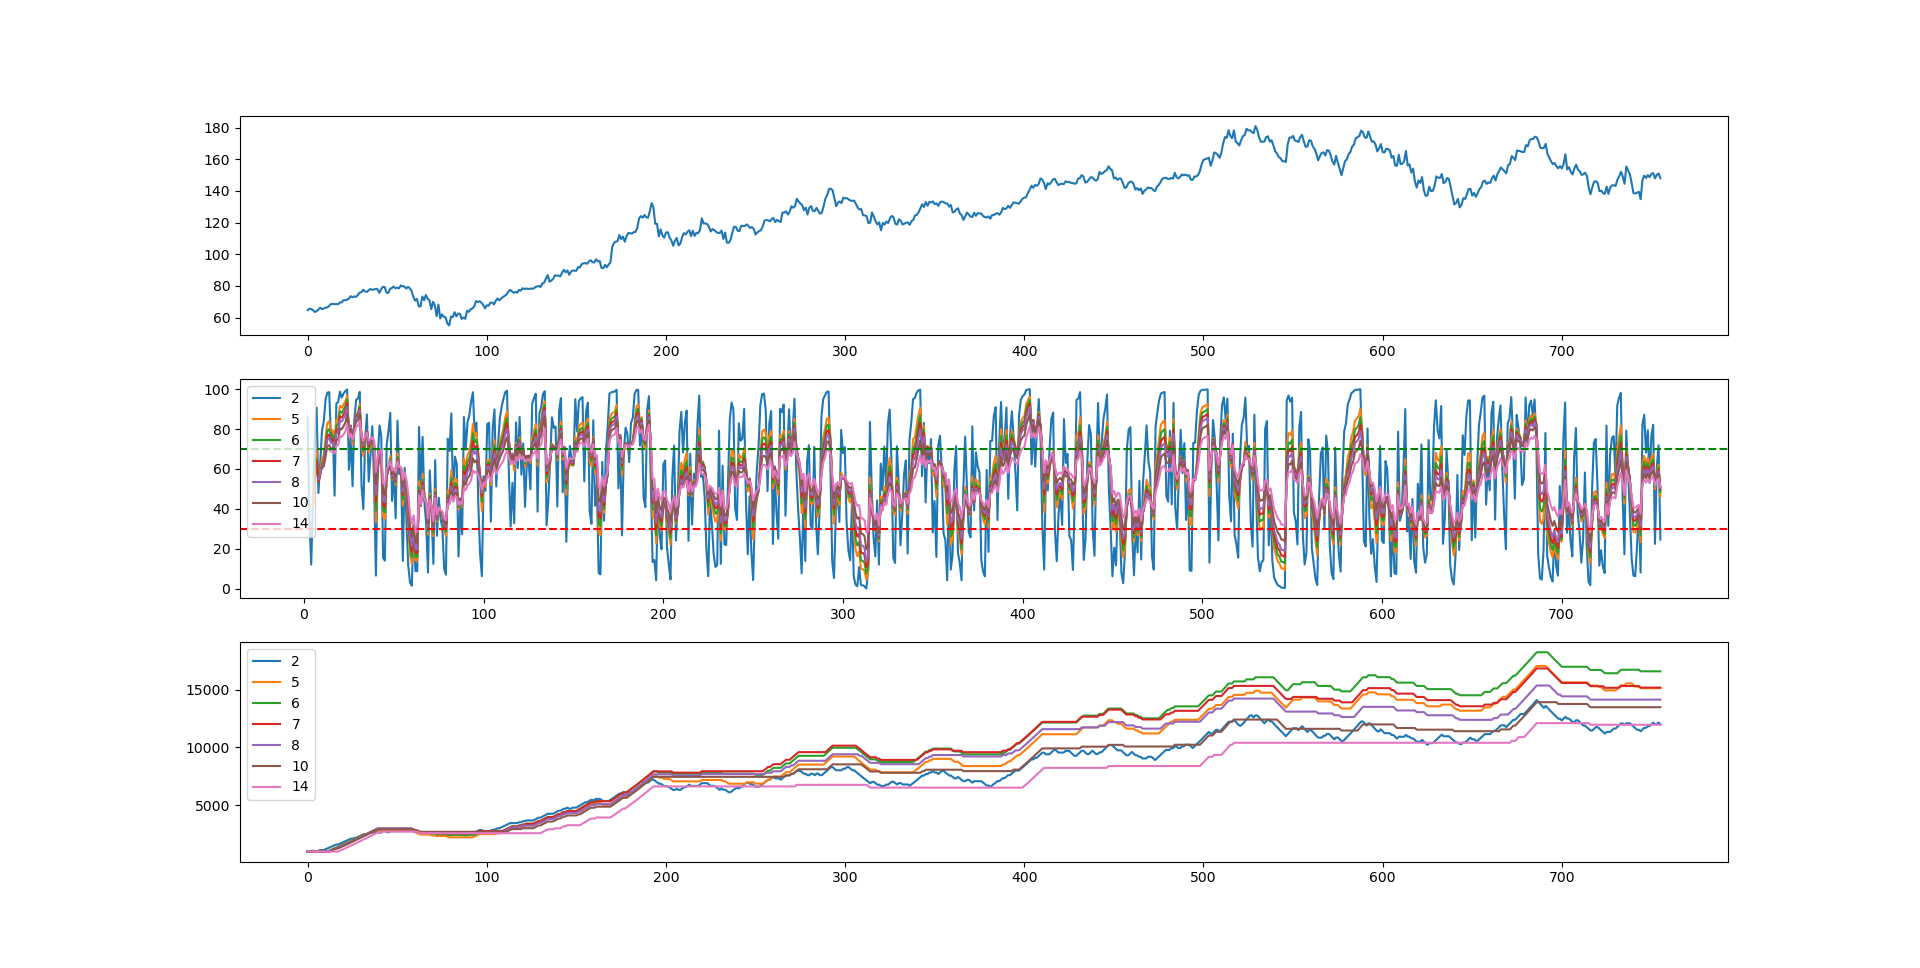
\includegraphics[width=\linewidth]{AAPL_3y.png}
  \caption{Évolution du cours de l'action Apple (AAPL) sur 3 ans, indicateur RSI et argent non investi. En légende, période de calcul du RSI}
  \label{fig:aaplrsi}
\end{figure}

\begin{figure}[!h]
  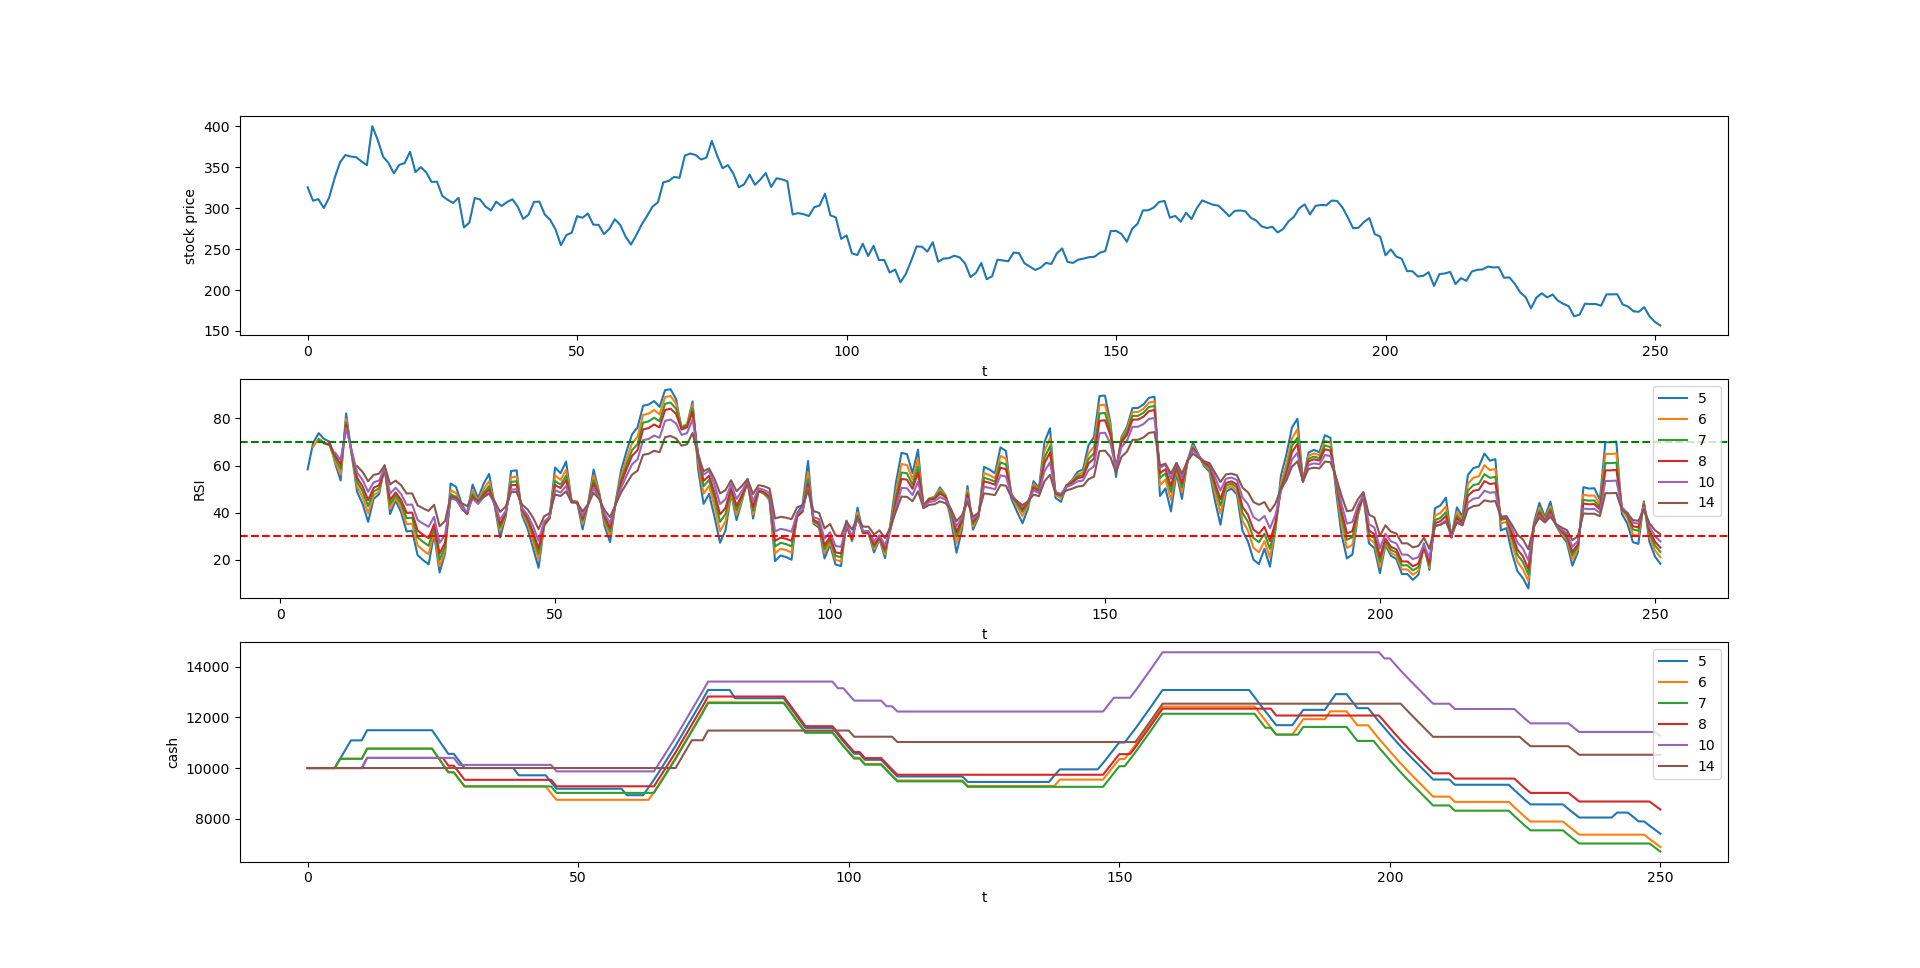
\includegraphics[width=\linewidth]{TSLA_1y.png}
  \caption{Évolution du cours de l'action Tesla (TSLA) sur 1 an, indicateur RSI et argent non investi. En légende, période de calcul du RSI}
  \label{fig:tslarsi}
\end{figure}

\twocolumn

\section{Implémentation du TDQN}

\href{https://github.com/pierrepebay/projet-ZZ2}{https://github.com/pierrepebay/projet-ZZ2}

\nocite{*}
\bibliographystyle{apalike}
\bibliography{citations}

\newpage

\end{document}
